\documentclass{standalone}
\usepackage{tikz}
\usepackage{pgfplots}



\tikzset{
  every point/.style = {circle, inner sep={.75\pgflinewidth}, opacity=1, draw, solid, fill=black},
  point/.style={insert path={node[every point, #1]{}}}, point/.default={},
  colored point/.style = {point={fill=#1}},
  point name/.style = {insert path={coordinate (#1)}},
  inherit/.style = {point/.style={insert path={node[circle, inner sep={.75\pgflinewidth}, draw, fill, #1]{}}}}
}

\begin{document}
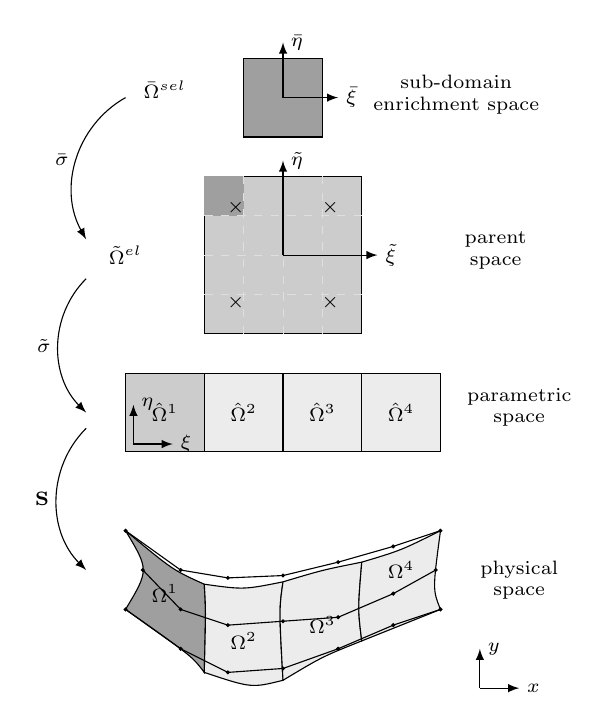
\begin{tikzpicture}
    [ subDomainQuad/.style={gray!75,draw=gray!75, fill=gray!75},
      activeQuad/.style={black,draw=black, fill=gray!40},
      inactiveQuad/.style={black,draw=black, fill=gray!15},
      grid/.style={very thin,gray!25,dashed},
      axis/.style={black,->,>=latex, thin},
      dim/.style={latex-latex}]
      
  \scriptsize




  %draw the subDomain enrichment space
  \draw[fill=gray!75]   (0,0) 
            		-- (+1.0,0) 
            		-- (+1.0,+1.0) 
            		-- (0,+1.0) 
            		-- cycle;

  \draw node at (-1.0, 0.6){$\bar{\Omega}^{sel}$};
  \draw node at (2.7, 0.7){sub-domain}; 
  \draw node at (2.7, 0.4){enrichment space}; 
            
  %draw the axes
  \draw[axis] (0.5,0.5) -- ++(0.7,0) node[anchor=west]{$\bar{\xi}$};
  \draw[axis] (0.5,0.5) -- ++(0,0.7) node[anchor=west]{$\bar{\eta}$};
  
  \draw[axis] (-1.5,0.5) to [bend right=45] node[left,midway]{$\bar{\sigma}$} (-2.0,-1.3) ;
  
  %draw the parent space
  \draw[activeQuad]   (-0.5,-2.5) 
                  -- (+1.5,-2.5) 
            		 -- (+1.5,-0.5) 
           		 -- (-0.5,-0.5) 
            		 -- cycle;
            		 
    \draw[subDomainQuad]   (-0.5,-1.0) 
            		-- (0.0,-1.0) 
            		-- (0.0,-0.5) 
            		-- (-0.5,-0.5) 
            		-- cycle;
            
  \draw node at (-1.5, -1.5){$\tilde{\Omega}^{el}$};
  \draw node at (3.2, -1.3){parent}; 
  \draw node at (3.2, -1.6){space}; 
    
  %draw gauss points
  \draw node at (-0.1,-0.9){$\times$};
  \draw node at (-0.1,-2.1){$\times$};
  \draw node at (1.1,-0.9){$\times$};
  \draw node at (1.1,-2.1){$\times$};


  %draw base mesh
   \begin{scope}

      \foreach \x in {0.0,0.5,...,1.0} 
      {
        \draw[grid] (\x,-2.5) -- ++(0.0,2.0);
      }

      \foreach \y in {-2.0,-1.5,...,-1.0} 
      {
        \draw[grid] (-0.5,\y,0.0) -- ++(2.0,0.0,0.0);
      }

   \end{scope}
   
  %draw the axes
  \draw[axis] (0.5,-1.5) -- ++(1.2,0) node[anchor=west]{$\tilde{\xi}$};
  \draw[axis] (0.5,-1.5) -- ++(0,1.2) node[anchor=west]{$\tilde{\eta}$};

  \draw[axis] (-2.0,-1.8) to [bend right=45] node[left,midway]{$\tilde{\sigma}$} (-2.0,-3.5) ;
  %draw the parameter space
  \draw[activeQuad]   (-1.5,-4.0) 
                  -- (-0.5,-4.0) 
            		 -- (-0.5,-3.0) 
           		 -- (-1.5,-3.0) 
            		 -- cycle;
            		 
  \draw node at (-1.0, -3.5){$\hat{\Omega}^{1}$};

  \draw[inactiveQuad]   (-0.5,-4.0) 
                  -- (0.5,-4.0) 
            		 -- (0.5,-3.0) 
           		 -- (-0.5,-3.0) 
            		 -- cycle;
   \draw node at (0.0, -3.5){$\hat{\Omega}^{2}$};
           		 
            		   \draw[inactiveQuad]   (0.5,-4.0) 
                  -- (1.5,-4.0) 
            		 -- (1.5,-3.0) 
           		 -- (0.5,-3.0) 
            		 -- cycle;
  \draw node at (1.0, -3.5){$\hat{\Omega}^{3}$};
            		 
            		   \draw[inactiveQuad]   (1.5,-4.0) 
                  -- (2.5,-4.0) 
            		 -- (2.5,-3.0) 
           		 -- (1.5,-3.0) 
            		 -- cycle;
            		 
  \draw node at (2.0, -3.5){$\hat{\Omega}^{4}$};
  \draw node at (3.5, -3.3){parametric}; 
  \draw node at (3.5, -3.6){space};  
  
  \draw[axis] (-1.4,-3.9) -- ++(0.5,0) node[anchor=west]{$\xi$};
  \draw[axis] (-1.4,-3.9) -- ++(0,0.5) node[anchor=west]{$\eta$};

  \draw[axis] (-2.0,-3.7) to [bend right=45] node[left,midway]{$\mathbf{S}$} (-2.0,-5.5) ;  
  %draw global space
  %Quad 1
  \draw[fill=gray!75]   (-1.5,-5.0) .. controls (-0.9,-5.5) .. (-0.5, -5.68) --
     (-0.5,-5.68) .. controls (-0.48,-6.0) .. (-0.5, -6.8) --
         (-0.5,-6.8) .. controls (-0.65,-6.6) .. (-1.5, -6.0)--
  (-1.5,-6.0) .. controls (-1.2,-5.5) .. (-1.5, -5.0);
	cycle;
  \draw node at (-1.0, -5.8){${\Omega}^{1}$};
	
  %Quad 2
  \draw[fill=gray!15]   (-0.5,-5.68) .. controls (0.0,-5.75) .. (0.5, -5.65) --
     (0.5,-5.65) .. controls (0.45,-6.0) .. (0.5, -6.9) --
         (0.5,-6.9) .. controls (0.1,-7.0) .. (-0.5, -6.8)--
  (-0.5, -6.8) .. controls (-0.48,-6.0) .. (-0.5,-5.68);
	cycle;
  \draw node at (0.0, -6.4){${\Omega}^{2}$};
	
 %Quad 3
  \draw[fill=gray!15]   (0.5,-5.65) .. controls (1.0,-5.5) .. (1.5, -5.4) --
     (1.5,-5.4) .. controls (1.45,-6.0) .. (1.5, -6.4) --
         (1.5, -6.4) .. controls (1.0,-6.6) .. (0.5, -6.9)--
    (0.5,-6.9) .. controls (0.45,-6.0) .. (0.5, -5.65);
	cycle;
  \draw node at (1.0, -6.2){${\Omega}^{3}$};
	
 %Quad 4
  \draw[fill=gray!15]   (1.5, -5.4) .. controls (2.0,-5.25) .. (2.5, -5.0) --
     (2.5,-5.0) .. controls (2.4,-5.75) .. (2.5, -6.0) --
         (2.5, -6.0) .. controls (2.0,-6.2) .. (1.5, -6.4)--
    (1.5,-6.4) .. controls (1.45,-6.0) .. (1.5,-5.4);
	cycle;
  \draw node at (2.0, -5.5){${\Omega}^{4}$};
	
  \draw node at (3.5, -5.5){physical}; 
  \draw node at (3.5, -5.8){space}; 
    
  %draw control points
  % first row
  \draw[thin, black] (-1.5,-5.0) [point] -- (-0.8,-5.5);
  \draw[thin, black] (-0.8,-5.5) [point] -- (-0.2,-5.6);
  \draw[thin, black] (-0.2,-5.6) [point] -- (0.5,-5.57);
  \draw[thin, black] (0.5,-5.57) [point] -- (1.2,-5.4);
  \draw[thin, black] (1.2,-5.4) [point] -- (1.9,-5.2);
  \draw[thin, black] (1.9,-5.2) [point] -- (2.5,-5.0)[point];
  % second row
  \draw[thin, black] (-1.28,-5.5) [point] -- (-0.8,-6.0);
  \draw[thin, black] (-0.8,-6.0) [point] -- (-0.2,-6.2);
  \draw[thin, black] (-0.2,-6.2) [point] -- (0.5,-6.15);
  \draw[thin, black] (0.5,-6.15) [point] -- (1.2,-6.1);
  \draw[thin, black] (1.2,-6.1) [point] -- (1.9,-5.8);
  \draw[thin, black] (1.9,-5.8) [point] -- (2.44,-5.5)[point];
  % third row
  \draw[thin, black] (-1.5,-6.0) [point] -- (-0.8,-6.5);
  \draw[thin, black] (-0.8,-6.5) [point] -- (-0.2,-6.8);
  \draw[thin, black] (-0.2,-6.8) [point] -- (0.5,-6.75);
  \draw[thin, black] (0.5,-6.75) [point] -- (1.2,-6.5);
  \draw[thin, black] (1.2,-6.5) [point] -- (1.9,-6.2);
  \draw[thin, black] (1.9,-6.2) [point] -- (2.5,-6.0)[point];
  
  \draw[axis] (3,-7) -- ++(0.5,0) node[anchor=west]{$x$};
  \draw[axis] (3,-7) -- ++(0,0.5) node[anchor=west]{$y$};
  
\end{tikzpicture}
\end{document}